Knowing structural properties of decomposable digraphs we first need to establish what a graph is.
A graph is a collection of nodes and edges between these nodes also called vertices which this report is going to use from now on.
we describe a graph $G(V,E)$ where $V$ and $E$ is two sets where $V$ is the set of vertices in the graph and $E$ is the set of edges in the graph.
Example $V=\lbrace a,b,c \rbrace$ then $a,b$ and $c$ are three distinct vertices of the graph $G$ and the only vertices of $G$ we denote the size of the graph as the number of vertices in the graph $|V|$.
In the case of the example the size of $G$ $|V|=3$ it is also called the order of a graph.
An edge is describe by the the two vertices it is connected to.
Thus $(a,b)$ is an edge between the vertex $a$ and $b$.
If an edge goes from and to the same vertex $(a,a)$ it is called a loop.
so the set of edges is describe whit $E=\lbrace (a,b),(a,a),(c,a),(c,b),(c,b)\rbrace$.
The describe example can be seen in figure \autoref{fig:graph}.
If we instead og an edges makes arcs we call it a digraph here the first vertex mentioned in an arc is the vertex from where the arc starts, the second is where the arc is going.
So the arc $(a,b)$ goes from $a$ to $b$, if you wanted it the other way around the arc is $(b,a)$.
these graph contaning only arcs and no edges is called a digraph which is what we in this project are focusing on.\\
\begin{figure}[!h]
    \centering
    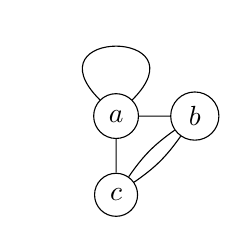
\begin{tikzpicture}
        [main/.style ={draw,circle}]
        \node[main] (a){$a$};
        \node[main] (b)[right of = a]{$b$};
        \node[main](c)[below of= a]{$c$};
        \draw (a) to (b) (c) to (a) (c) to [bend right =10](b) (c) to [bend left =10](b); 
        \draw (a) to [loop] (a);
    \end{tikzpicture} 
    \label{fig:graph}
    \caption{graph $G(V,E)$ used as an example of describing graphs in general}
\end{figure}


before delving into graphs and digraphs we must establish some important prerequisite and properties. 
A graph is simple is there is no loops and no multiple edges. 
With multiple edges it means multiple edges between the same pair of vertices.
A graph is called complete if there for all pair of vertices in the graph is an edge between them.\\
A graph is connected if there exists a path between all pair of vertices in the graph and disconnected otherwise.
a path in a graph is is a walk where a vertex is only passed onces.
A walk in a graph is a ordering of vertices an edges in the graph where the edge in between the vertex in the ordering is an edge between the vertices so for $a,e_1,b$ to be a walk the edge $e_1$ has to be between $a$ and $b$.

in a digraph a graph we have something called the underlying graph. 
An underlying graph of a digraph is where all arcs are replaced by edges (edge is used every time we talk about undirected edges between vertices, when direction is mentioned it is called an arc).
A digraph is connected if the underlying graph is connected, (also called weakly connected), a digraph can be strongly-connected and semi connected too.
A digraph is called semi connected if there for each pair $u$ and $v$ exists a path from either $u$ to $v$ or $v$ to $u$. 
It is said to be strongly connected if for each pair of vertices $u$ and $v$ there exists a path from both $u$ to $v$ and $v$ to $u$.

We can use these to describe som specific collection of graphs as the graph tournaments.
tournaments is a digraph where the underlying graph is complete. 
An underlying graph of a digraph is where all arcs are replaced by edges (edge is used every time we talk about undirected edges between vertices, when direction is mentioned it is called an arc).
So a complete graph of order 5 any orientation of the edges concludes in a tournament.
If instead of replacing the one edge by one arc in either direction, but instead replace it by two arcs the digraph is called semicomplete.

The reason for grouping the digraphs into smaller collections of digraphs (like tournaments is a smaller collection of semicomplete digraphs) is because of problems is easy describe on specific graphs than general graphs.

We have these graph called NP-hard problems which sometimes sound easy solvable for graphs but only for some specific graphs we know how to solve it in polynomial time. 
\begin{definition}
    define NP-hard problems
\end{definition}

In this paper we focusing on the specific digraphs that are decomposable. 
A decomposable digraph is a digraph $D=H[G_1,G_2,\dots,G_|H|]$ where each $G_i$ is disconnected graphs replacing each vertex of the digraph $H$. ...
